\documentclass[]{article}
\usepackage{lmodern}
\usepackage{amssymb,amsmath}
\usepackage{ifxetex,ifluatex}
\usepackage{fixltx2e} % provides \textsubscript
\ifnum 0\ifxetex 1\fi\ifluatex 1\fi=0 % if pdftex
  \usepackage[T1]{fontenc}
  \usepackage[utf8]{inputenc}
\else % if luatex or xelatex
  \ifxetex
    \usepackage{mathspec}
  \else
    \usepackage{fontspec}
  \fi
  \defaultfontfeatures{Ligatures=TeX,Scale=MatchLowercase}
\fi
% use upquote if available, for straight quotes in verbatim environments
\IfFileExists{upquote.sty}{\usepackage{upquote}}{}
% use microtype if available
\IfFileExists{microtype.sty}{%
\usepackage{microtype}
\UseMicrotypeSet[protrusion]{basicmath} % disable protrusion for tt fonts
}{}
\usepackage[margin=1in]{geometry}
\usepackage{hyperref}
\hypersetup{unicode=true,
            pdftitle={Researchers' perceptions of malaria eradication: findings from a mixed-methods analysis of a large online survey},
            pdfborder={0 0 0},
            breaklinks=true}
\urlstyle{same}  % don't use monospace font for urls
\usepackage{longtable,booktabs}
\usepackage{graphicx,grffile}
\makeatletter
\def\maxwidth{\ifdim\Gin@nat@width>\linewidth\linewidth\else\Gin@nat@width\fi}
\def\maxheight{\ifdim\Gin@nat@height>\textheight\textheight\else\Gin@nat@height\fi}
\makeatother
% Scale images if necessary, so that they will not overflow the page
% margins by default, and it is still possible to overwrite the defaults
% using explicit options in \includegraphics[width, height, ...]{}
\setkeys{Gin}{width=\maxwidth,height=\maxheight,keepaspectratio}
\IfFileExists{parskip.sty}{%
\usepackage{parskip}
}{% else
\setlength{\parindent}{0pt}
\setlength{\parskip}{6pt plus 2pt minus 1pt}
}
\setlength{\emergencystretch}{3em}  % prevent overfull lines
\providecommand{\tightlist}{%
  \setlength{\itemsep}{0pt}\setlength{\parskip}{0pt}}
\setcounter{secnumdepth}{0}
% Redefines (sub)paragraphs to behave more like sections
\ifx\paragraph\undefined\else
\let\oldparagraph\paragraph
\renewcommand{\paragraph}[1]{\oldparagraph{#1}\mbox{}}
\fi
\ifx\subparagraph\undefined\else
\let\oldsubparagraph\subparagraph
\renewcommand{\subparagraph}[1]{\oldsubparagraph{#1}\mbox{}}
\fi

%%% Use protect on footnotes to avoid problems with footnotes in titles
\let\rmarkdownfootnote\footnote%
\def\footnote{\protect\rmarkdownfootnote}

%%% Change title format to be more compact
\usepackage{titling}

% Create subtitle command for use in maketitle
\newcommand{\subtitle}[1]{
  \posttitle{
    \begin{center}\large#1\end{center}
    }
}

\setlength{\droptitle}{-2em}
  \title{Researchers' perceptions of malaria eradication: findings from a
mixed-methods analysis of a large online survey}
  \pretitle{\vspace{\droptitle}\centering\huge}
  \posttitle{\par}
  \author{}
  \preauthor{}\postauthor{}
  \date{}
  \predate{}\postdate{}

\usepackage{multicol}
\usepackage{hyperref}
\usepackage{geometry}
\usepackage[utf8]{inputenc}
% \usepackage[T1]{fontenc}
\usepackage{lmodern}
\usepackage{etoolbox}
% \AtBeginEnvironment{quote}{\singlespacing\small}
% \usepackage{setspace} % for \onehalfspacing and \singlespacing macros
% \onehalfspacing 

\usepackage{fancyhdr} % Headers and footers
\pagestyle{fancy} % All pages have headers and footers
\fancyhead{} % Blank out the default header
\fancyfoot[C]{\thepage} % Blank out the default footer
\fancyhead[C]{ $\bullet$ Manuscript submission to SSM $\bullet$ } 
\renewcommand{\thefootnote}{\fnsymbol{footnote}}

\newcommand{\footremember}[2]{%
    \footnote{#2}
    \newcounter{#1}
    \setcounter{#1}{\value{footnote}}%
}
\newcommand{\footrecall}[1]{%
    \footnotemark[\value{#1}]%
} 

\def\changemargin#1#2{\list{}{\rightmargin#2\leftmargin#1}\item[]}
\let\endchangemargin=\endlist 

\usepackage{soul}

\usepackage{setspace}
\doublespacing

\usepackage[right, modulo]{lineno}
\linenumbers

\begin{document}
\maketitle

\begin{center}
\textbf{Abstract}  
\end{center}

\vspace{5mm}

\begin{center}
\begin{changemargin}{3cm}{3cm} 

Quantifying an event's probability and time frame is essential for calculating its expected value. Uncertainty regarding feasibility makes it difficult for policymakers and public health practitioners to forecast the return on investment of malaria eradication. Since the opportunity cost of investments in eradication-specific interventions can be high - particularly in contexts with other urgent health priorities - understanding eradication's expected value is essential. In a large online survey of malaria researchers (n = 844), we query perceptions regarding the likelihood and time frame of eradication. We assess perceived years to and likelihood of eradication, and adjust for selection bias. We also carry out a qualitative analysis of the free-form comments provided by 61\% of respondents. Our results show that researchers are skeptical of the feasibility of near-term malaria eradication, with most believing that eradication will not be achieved for 50 years or more.
\end{changemargin}
\end{center}

\vspace{10mm}

\noindent\fbox{%
    \parbox{\textwidth}{%
        \subsection*{Research Highlights}
        \begin{itemize}
          \item Employs a very large online survey of specialist researchers
          \item Assesses perceived time frame and likelihood of global malaria eradication among researchers
          \item Results suggest that most malaria researchers believe short-term global malaria eradication to be unlikely
          \item Identifies challenges pertaining to eradication through qualitative analysis
        \end{itemize}
      \subsection*{Keywords}
        Malaria; eradication; elimination; mixed methods; survey; crowdsourcing 
    }%
}

\newpage

\section{Introduction}\label{introduction}

\subsection{Background}\label{background}

Malaria is a parasitic disease transmitted among humans by mosquitoes.
The \emph{Plasmodium falciparum} species accounts for a large majority
of the 200 million annual cases as well as the half million annual
deaths worldwide (White et al., 2014) (WHO, 2016) (Ashley et al., 2018).
Malaria ``elimination'', the ``interruption of all local transmission of
the infection in a country or region'' (Tanner et al., 2015) is actively
being pursued by dozens of countries around the world, leading to a
renewed push for ``eradication'' (``the worldwide interruption of
transmission'') (Hopkins, 2013) (Rabinovich et al., 2017) (Lancet,
2011).

This is not the first time that eradication has been in the
international spotlight. The scientific and public health communities
have had eradication on their policy agenda since the World Health
Organisation (WHO) established the Global Malaria Eradication Program in
the 1950s (Nájera et al., 2011). In 1957, U.S. President Dwight
Eisenhower told Congress that malaria could be expected to be eradicated
in five years. Following the failure of the WHO's first attempt, the
focus shifted away from global eradication towards local elimination and
control strategies. In recent years, much of the discourse regarding
malaria has shifted back to global eradication (Roberts and Enserink,
2007), with funders, researchers, and public health practitioners
rallying to the cause (Tanner et al., 2015). The Bill and Melinda Gates
Foundation has begun actively promoting eradication as feasible ``within
a generation'' (Gates, 2014), and the WHO has set ambitious goals,
stating the objective of eliminating malaria in 65 new endemic countries
from 2015 through 2030 (Figure 1).

\begin{figure}[h]

{\centering 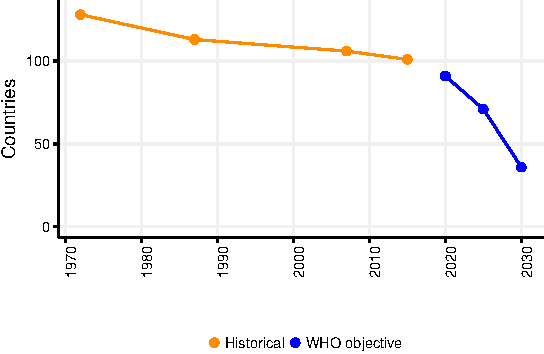
\includegraphics{paper_files/figure-latex/unnamed-chunk-3-1} 

}

\caption{Countries with malaria: Observed and WHO objectives}\label{fig:unnamed-chunk-3}
\end{figure}

Even in areas of high endemicity, advances in immunology, parasitology,
modeling and vaccinology, along with rapid economic development, have
made eradication appear a more feasible goal, though not possible in the
short term (Snow, 2015) (Eckhoff et al., 2014). From both administrative
(Yamey, 2004) and scientific (Alonso et al., 2011) points of view,
eradication has never before received so much attention.

Most of the current research on expert opinion regarding the feasibility
of malaria eradication focuses on the \emph{how} rather than the
\emph{if} and the \emph{when} (Tanner et al., 2015). The participants in
the Malaria Eradication Research Agenda (MalERA) process, in particular,
have guided research goals and identified gaps in order for elmination
to occur (Alonso et al., 2011) (Rabinovich et al., 2017). Though the
MalERA authors firmly state that eradication is \emph{not} feasible
given the ``current tools and state of knowledge'', mentions to the time
frame are vague (``within the lifetime of young scientists just
embarking on their careers'' (Alonso et al., 2011) and ``in the longer
term'' (Rabinovich et al., 2017)) and no mention is made of the
perception of the overall probability of achieving eradication.
International programmes, such as the WHO Global Malaria Programme
(GMP), have acknowledged the need ``to take an official position on how
and under what timeline malaria eradication could be achieved''
(``Malaria policy advisory committee to the WHO,'' 2015). Clarity on
timeline and likelihood of eradication could inform forecasting of
disease transmission, and plays a crucial role in the economic analysis
of the expected value of malaria eradication initiatives, ultimately
informing health policy decisions. But achieving clarity is difficult,
given the many complex and interacting variables which affect malaria
transmission, research funding, and technological development. The
question of \emph{how} is complex enough, rendering questions of
\emph{if} and \emph{when} even more difficult to answer.

Proponents of disease eradication point to the success of historical and
current campaigns (smallpox and polio, respectively), and highlight the
long term benefits in health and wealth to future generations (Barrett,
2013). One often cited figure is for smallpox eradication, in which the
investment of each dollar led to a return of greater than 400 (Barrett,
2006); unlike smallpox (for which analysis was able to be
retrospectively constructed based on observed costs and benefits), in
the case of a prevalent disease, forecasting models have to be used in
order to prospectively estimate the value of an investment. Additionally
the estimated impact of malaria on economic indicators is heterogeneous,
with singificant impact in areas of Sub-Saharan Africa - where the
endemicity is high - and little to no impact in areas of low endemicity
(Cutler et al., 2010) (Barofsky et al., 2015).

The general objective of eradication serves to inspire, rally funder
support, motivate researchers, and focus the efforts of public health
practitioners. The recently established Lancet Commission on malaria
eradication states that ``eradication is the only acceptable end goal''
(while acknowledging that there exists ``scepticism about {[}its{]}
technical feasibility'') (Chen et al., 2018). To the extent that malaria
eradication (by definition) has never occurred, the parameters needed
for a ex-post cost-benefit analysis are unknown. Nonetheless,
prospectively estimating eradication's return on investment is crucial
to deciding when and how to pursue the goal, especially in light of the
high direct and opportunity costs of eradication-specific interventions.
One approach to economic evaluation is the use of mathematical and
stochastic models. These have been applied to diseases which are closer
to eradication than malaria, since the uncertainty around model input
parameters is less, requiring fewer cascading assumptions in order to
present possible comparative scenarios. For example, Kastner et al. were
able to describe 4 relatively realistic pathways to Lympathic Filariasis
eradication, as well as the pre-requisite role and magnitude of certain
interventions (Kastner et al., 2015). A similar modeling framework was
then used to estimate the cost of eradication (Kastner et al., 2017). A
recent modeling analysis on onchocerciasis eradication, based on a
disease transmission model, showed that the costs of elimination
(relative to staying in ``control mode'') in Africa would be far lower
even in the short term, thanks to the improvements it would lead to in
both treatment times and prevented surveillance costs. Given the
relative proximity of eradication, and the narrow geographic scope, the
authors were also able to estimate the timeline to eradication (Kim et
al., 2017).

This level of detail and specificity in the economic evaluation
landscape of malaria eradication, unfortunately, is not possible (or at
least not commonly undertaken), given its high prevalence and
epidemiological complexity. In fact, there are no mathematical models
(to the authors' knowledge) estimating the likelihood and time frame of
eradication, or its derivative cost-benefit ratio. Globally, where
mathematical modeling has been used for the purposes of forecasting the
future epidemiology of malaria, the methods have generally been aimed at
optimizing elimination methods (Slater et al., 2015), determining
whether a strategy is scalable (Brady et al., 2017), guiding funding and
drug development (Patouillard et al., 2017) (Slater et al., 2017), or
comparing a range of hypothetical morbidity scenarios (Winskill et al.,
2017), rather than assessing the likelihood of or time until the
occurrence of those scenarios.

To the extent that (i) estimating eradication's likelihood and timeframe
is essential to forecasting the cost-benefit ratio of eradication
interventions, and (ii) mathematical models generally do not venture
into areas of such high uncertainty, alternative methods are needed.
Just as the stock market aggregates perceptions to provide a fairly
accurate assessment of something as complex as a company's value,
aggregating perceptions may be a useful tool for tackling the complexity
of malaria eradication. Many studies have shown value in expert
elicitation as a means to reduce uncertainty and inform decision making
(Morgan, 2014). As Francis Galton demonstrated in his famous study in
which he showed that the crowds' aggregated estimates of cow's weight
formed a quasi-normal distribution centered around the true weight
(Wallis, 2014) (Galton, 1907), averaging the perceptions of many can be
more accurate than taking the opinion of any single expert, since the
biases of diverse viewpoints can be complementary and symbiotic.
Measuring consensus and discord among disease-specific researchers from
a variety of disciplines can serve as a barometer of (informed) opinion,
both guiding resources and identifying areas of concern (Keenan et al.,
2013).

The optimal assignment of resources for malaria eradication campaigns
hinges on the expected value of those campaigns, the latter being a
direct function of the discount rate applied to future benefits and the
probability of ``success'' (ie, eradication). Holding constant factors
such as the cost of eradication and the benefits of achieving it, the
return on investment of malaria eradication initiatives is a function of
eradication's timeframe (assuming a \textgreater{} 0 discount rate) and
probability (assuming a \textless{} 100\% likelihood of success). Given
this, estimating these parameters is crucial to evaluating if and when
attempts at eradication should be undertaken.

Though the case-specific marginal cost of eradication can be expected to
be high (relative to a simple control approach), successful eradication
would mean massive recurring savings in the long-term (Barrett, 2013).
However, to the extent that the case-specific marginal cost of
prevention in an eradication campaign is high, estimating the likelihood
of success is fundamental to the correct distribution of resources,
particularly in low-income environments.

We propose that the aggregation of malaria researchers' perceptions
regarding the time frame and likelihood of eradication forms a
probability distribution which can be used to estimate the expected
value of eradication-specific investments. The objective of this study
is to gauge (expert) opinion about, estimate the likelihood of, and
quantify the potential time frame to malaria eradication through a
systematic online survey of malaria research professionals from a wide
array of academic disciplines. In doing so, we aim to help guide the
optimal distribution of health resources by informing estimations of the
expected value of malaria eradication efforts.

\section{Methods}\label{methods}

Our study population included all first authors (with available email
addresses) returned in a PubMed search for the term ``malaria'' from
January 1, 2010 through December 20, 2016. We used PubMed because it was
the most comprehensive publication database for malaria-releated
research, and also exposed enough metadata about articles and authors so
as to allow for relevant analysis. Personalized emails addressing the
author by name and mentioning the relevant paper were sent to each of
the 7680 authors during the period from December 20, 2016 through
January 2, 2017. Researchers were invited to participate by clicking a
link to the survey form. The survey was simple, consisting of only name,
email, and four content-related fields along with a ``general comments''
section. The survey was administered and data were collected through
Google Drive. The original survey is viewable at
\url{https://goo.gl/forms/IroAEooDuJ6KM5Ho2}.

Content-related survey fields consisted of:

\begin{enumerate}
\def\labelenumi{\arabic{enumi}.}
\tightlist
\item
  Area of expertise.
\item
  Perceived probability (\%) of malaria eradication in 10, 20, 30, 40,
  and 50 years.
\item
  Free choice perceived number of years until malaria eradication.
\end{enumerate}

The survey was intentionally as short as possible, so as to appeal to
time-pressed participants. However, supplementary data on researchers is
of value for the assessing of selection bias and determinants of
perception. Accordingly, we estimated the likelihood of a participant
being of one of two genders (male or female) based on first name. In
order to do this, we used data from the North Atlantic Population
Project, and U.S. government (Mullen, 2015). We also calculated the
total number of citations which each author had received, as well as the
total number of articles authored. We binned total citations into three
categories: 0-5 (junior-level researchers, PhD students, etc.); 6-99
(most professional academics); and \textgreater{}99 (the most prolific
researchers). The searching and retrieval of information pertaining to
articles and citations from the PubMed database was carried out using
the RISmed package (Kovalchik, 2015). Information retrieved about
authors was used to de-bias paramaters in an ordinary least squares
regression, analyzing the association between number of publications and
perceived years to eradication.

Survey results were first analyzed descriptively. Following Francis
Galton's example, we naively take the average of all responses as the
likely point estimate for event probabilities, and the totality of the
responses to each numeric question as the likely confidence interval of
those likelihoods and time frames.

Quantitative analysis was carried out in R language (R Core Team, 2015).
All analysis code, as well as the code used for the identification and
contacting of participants, is publicly available at
\url{https://github.com/joebrew/malaria_survey}.

Qualitative analysis of free text comments was carried out using
thematic content analysis, with inductive open coding (Markey et al.,
2014). Participants were invited to provide ``any general comments on
the timeline and likelihood of global eradication''. Thematic content
analysis (Vaismoradi et al., 2016) was employed to code responses
following the 6-phase approach laid out by Braun and Clarke (Braun and
Clarke, 2006). The approach was inductive, used open-coding to identify
latent themes, and underwent several iterations in which codes were
modified, discarded and created. Using the RQDA software to assist in
data management and theme coding (Huang, 2017), four subject themes were
identified. Comments were additionally coded as either descriptive
(comments pertaining to the ``problem'' of malaria eradication) or
presciptive (pertaining to potential ``solutions'' for eradicating
malaria). Finally, free-text comments were scored for overall sentiment
polarity (Rinker, 2017).

\section{Results}\label{results}

\begin{figure}[h]

{\centering 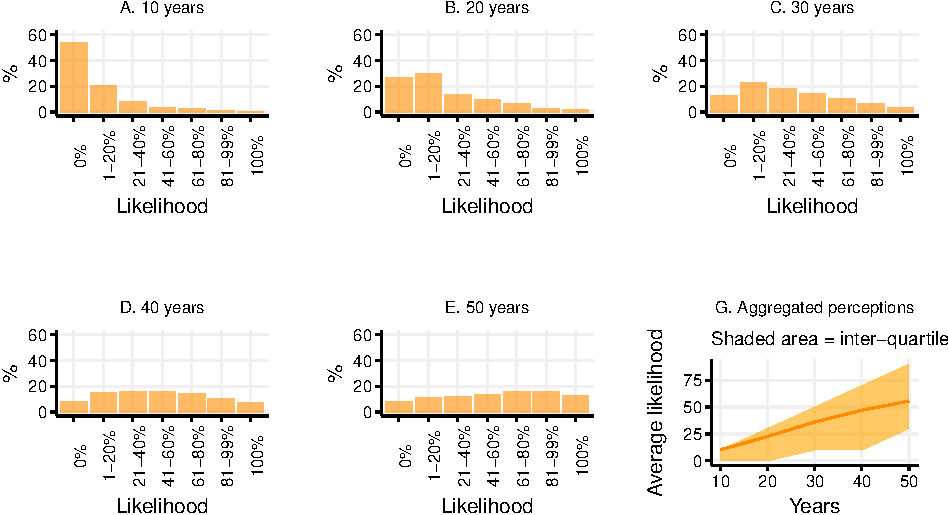
\includegraphics{paper_files/figure-latex/unnamed-chunk-4-1} 

}

\caption{Perceptions of likelihood of eradication}\label{fig:unnamed-chunk-4}
\end{figure}

A total of 884 researchers participated in the survey from the 7918
invitations sent (participation rate of 11.16\%). Areas of expertise
were non-exclusive and self-described, with participants having the
option to choose from up to 3 of 10 checkboxes, or to write in one or
more ``other'' areas of
expertise.\footnote{Response categories were Anthropology, Biochemistry, Bioinformatics, Biology, Chemistry, Clinical medicine, Drug discovery, Ecology, Economics, Entomology, Epidemiology, Geography, GIS, History, Immunology, Infectious disease, IT, Malaria, Medical entomology, Medicinal chemistry, Microbiology, Parasitology, Pharmacology, Pharmacy, Political science, Public health, Statistics, Vector biology, Vector control, and Virology.}
604 (68.3\%) participants declared three or fewer areas of expertise.

Participants had a total of 219 unique (self-described) areas of
expertise. The five most popular were Epidemiology (357), Information
Technology (344), Parasitology (319), Biology (277), Clinical medicine
(207).

\subsection*{Quantitative results}

Most participants saw eradication as extremely unlikely in the next
10-30 years, but increasingly likely thereafter. Figure 2 shows the
distribution of year-specific likelihood perceptions (panels A-E), as
well as an illustration of how both likelihood and uncertainty grow over
time (panel F). At the 40 year mark, the distribution of perceived
likelihood of eradication appears ``normal'', and by 50 years it is
slightly shifted to the right (ie, consensus is towards eradication more
probable than not).

In regards to responses to perceived years until eradication, 59 (0.7\%)
were either blank or uninteligible, whereas 825 participants responded.
Among respondants, 616 (74.7 \%) estimated that it would be 50 or more
years until eradication.

Respondents were qualitatively different from non-respondents.
Importantly, the average number of total author-specific citations was
40.91 among respondents, but 92.92 among non-respondents. This suggests
a tendency for more senior or impactful researchers not to respond. When
examining the number of average citations per article, the difference
between respondents remained: 4.75 among respondents, and 8.95 among
non-respondents, highlighting the greater impact of non-respondents
relative to respondents. Males responded at a greater rate (12.18) than
females (9.14).

\begin{longtable}[]{@{}llrrl@{}}
\caption{Response rate by author characteristics}\tabularnewline
\toprule
Variable & Characteristic & Responded & Invited & Response
rate\tabularnewline
\midrule
\endfirsthead
\toprule
Variable & Characteristic & Responded & Invited & Response
rate\tabularnewline
\midrule
\endhead
Sex & Female & 209 & 2287 & 9.14 \%\tabularnewline
& Male & 358 & 2939 & 12.18 \%\tabularnewline
& NA & 317 & 2692 & 11.78 \%\tabularnewline
Citations & 0-5 & 621 & 3299 & 18.82 \%\tabularnewline
& 6-99 & 179 & 3270 & 5.47 \%\tabularnewline
& \textgreater{} 99 & 84 & 1349 & 6.23 \%\tabularnewline
\bottomrule
\end{longtable}

Selection bias is not of concern in the case of differential response if
the groups for whom there are differences are not different in terms of
the outcome variable. This was the case for sex: males responded at a
significantly greater rate than females (p \textless{} 0.001), but were
not statistically significantly different in regards to
pessimism/optimism (ie, time frame or likelihood of eradication). In the
case of researcher impact (as measured by the total number of
citations), selection bias plays an important role: being highly-cited
was associated both with eradication ``pessimism'' as well as likelihood
of non-response. In other words, our pool of respondents was less
highly-cited than our pool of invitees, and among respondents, those who
were highly-cited tended to be more pessimistic.

In order to de-bias sample selection, we employed Heckman's two-step
correction method as well as simple binomial logistic regression model
to estimate the likelihood of response as a function of sex and (binned)
number of citations. To the extent that the two methods presented nearly
identical value, we present here the results of the latter. Having
estimated the odds of survey participation, we then used the inverse of
the selection model's predictions as weights in a simple linear model to
adjust our estimates. We run a separate weighted model to estimate the
likelihood of eradication at 10, 20, 30, 40, and 50 years. Figure 3
shows both the aggregated perceived likelihood of eradication over time
before and after adjusting for sample selection based on binned number
of publications. Our adjusted and unadjusted estimates coincide in the
long-term, but diverge sharply in the near-term; adjustment suggests
that had our pool of respondents been more representative, the average
perceived likelihood of near-term eradcation would have been much lower.

\begin{figure}[h]

{\centering 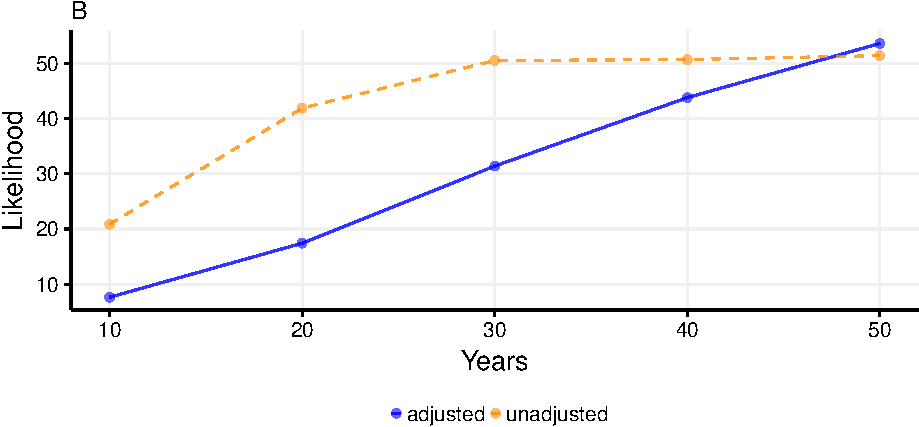
\includegraphics{paper_files/figure-latex/unnamed-chunk-10-1} 

}

\caption{Aggregated perceived likelihood of eradication over time, adjusted for sample selection and unadjusted.}\label{fig:unnamed-chunk-10}
\end{figure}

\subsection{Qualitative analysis of
comments}\label{qualitative-analysis-of-comments}

Of the 884 who responded to the survey, 540 (61.09\%) provided a
comment. Relative to non-commenters, commenters were more optimistic on
average, but also more polarized in opinion. The three subject themes
identified through iterative, open coding were:

\begin{enumerate}
\def\labelenumi{\arabic{enumi}.}
\item
  \emph{Solutions}: Comments pertaining to the innovations required to
  achieve eradication, priorities, and the desirability of certain
  approaches.
\item
  \emph{Systemic challenges}: comments pertaining to political, social,
  environmental or logistical issues related to eradication.
\item
  \emph{Complexity}: comments which focus on the multi-dimensional
  components of eradication.
\end{enumerate}

Comments were also classified as descriptive or prescriptive. A majority
(59.26\%) were descriptive. Descriptive commenters were more pessimistic
(in regards to perceived years until eradication) than prescriptive
commenters, though this difference did not reach the level of
statistical significance (p = 0.21 using Pearson's Chi-squared test).
Descriptive comments also received sentiment polarity scores which were
more negative than prescriptive comments, although again this difference
did not reach the level of statistical significance (p = 0.18).

In regards to \textbf{solutions}, comments largely pertained to the
necessity of further technological advances and innovations. One
participant wrote that ``currently available technology can't achieve
{[}eradication{]}, even if delivered optimally''; another argued that
eradication could not be achieved without a ``game-changing
innovation'', whereas multiple others referred to the need for
``transformative'' technologies:

\begin{quote}
We can't achieve eradication with our current tools. We'd need new medicines, a better vaccine, and maybe other vector control tools.
\end{quote}

Many noted the need to ``overcome the challenge of drug resistance''.
More than 10\% of commenters noted the need for an effective vaccine.
Genetic engineering was mentioned by several commenters as a promising
means to achieve eradication quickly. Most comments coded as
``solutions'' were presciptive in nature, often suggesting the nature of
the needed innovation, with a heavy slant towards pharmaceutical options
and vaccination.

\textbf{Systemic challenges} to malaria eradication were noted by the
majority of commenters. Comments in this category can be divided into
four sub-themes: (i) lack of coordination, (ii) lack of good
surveillance and health services delivery, (iii) lack of political will
and (iv) poverty. In direct contrast to the previous comments, many
emphasized that ``we already have the tools to achieve eradication'' and
that the only piece lacking was ``robust health systems''. Many
commenters noted problems of coordination, as illustrated in the below
quote.

\begin{quote}
It will be very difficult to eradicate malaria... not because we don't have the technologies, which we already have... the problem is politics. Malaria doesn't stop in (sic) borders of a country and it would take a joint effort of a lot of political leaders to get programs in place to fight malaria. Unfortunately I don't see this happening anytime soon.
\end{quote}

Others echoed the sentiment, with many comments focusing on the need of
strong surveillance and treatment delivery systems. Many commenters
focused on other reasons for stagnating progress, such as ``weak or
failing health systems\ldots{}due to political unwillingness or
conflict''. Many noted that malaria is a ``disease of poverty'', with
``social injustice'' as the root cause. Some made the sequential
argument that ``eradication of poverty'' must preceed disease
eradication. Along the same lines, one commenter wrote:

\begin{quote}
Eradication requires a full systems-wide approach, not a disease-specific approach. The eradication of smallpox was a triumph of management, not medicine or technology.
\end{quote}

Another noted that the survey ``left off the list the most important
factor - economic development''. Many echoed the sentiment, stating that
``with no economic development, you cannot have eradication'' and that
poverty is the ``cause'' of malaria. Comments coded as ``systemic''
tended to be descriptive and more pessimistic than others.

\textbf{Complexity} was a relatively rare category (\textless{}20\% of
all comments), those whose comments were coded as the ``complexity''
category were more pessimistic than average in regards to the timeline
and likelihood of eradication. Many commenters highlighted the inherent
challenges in the epidemiology of malaria, such as the changing dynamics
of malaria transmission, the resilience of the parasite and vector,
climate change, and the inability to aim interventions accurately with
an ``ever-moving target''. The potential for adaptation was highlighted
in reference both to the mosquito as well as the parasite itself. Many
comments addressed the fact that the conversation on eradication is
largely taking place within the public health community, whereas the
causes of malaria endemicity are largely orthogonal to public health
interventions, ``going beyond the health sector''. Several commenters
pointed out the multitude of prerequisite conditions for eradication to
even be considered feasible:

\begin{quote}
To my mind, this question is highly dependent on background context, e.g. global political and economic dynamics, as well as international conflict. Complete global eradication is an extremely singular goal that requires a vast array of necessary conditions - if any of these fail, eradication will not be achieved.  
\end{quote}

Many commenters thought that the terms ``eradication'' and ``malaria''
were so complex and nebulous that the public health practitioners should
avoid the them all together, so as to not repeat the mistakes of the WHO
GMP in the 1950s. For example, some highlighted that talking about
``malaria'' as one disease misses the mark, since the different species
of parasite and contexts in which they live make elimination in each
area very distinct from other areas. One commenter wrote that
eradication is a ``postwar'' idea that developed from the ``abandonment
of a broad sociopolitical understanding of the causes of disease, and
the emphasis on technological solutions.'' Many stated that global
malaria eradication was simply not possible, and two argued that it may
not be desirable or ethical. One stated that the concept was ``absurd''
and that ``I'm not even sure why people talk about it''. Another
questioned the utility of discussing ``eradication'' as a concept:

\begin{quote}
Eradication is a different objective than elimination. Elimination means that the disease is not endemic but could reappear even in a country like Norway if infrastructure breaks down. Elimination may be possible in poor endemic countries, following socioeconomic development. Eradication means that the parasite disapears from the planet, which is not realistic...
\end{quote}

Comments questioning the utility of eradication as a concept or goal
tended to be skeptical of its feasibility. Largely, they were
prescriptive, advocating for a re-framing of the conversation so that
the focus was not on an ``arbitrary'' goal like eradication, but rather
on scaling up control and making region-specific progress.

\section{Discussion}\label{discussion}

Approximately three-quarters of respondents believe that malaria will
not be eradicated in the next 50 years. When adjusted for selection
bias, the perceived likelihood of eradication in 50 years remains
similarly low, but estimates for shorter-term eradication are even
lower.

Eradication of a disease is a ``high stakes game'', exposed to multiple
competing - and at times contradictory - incentives from multiple
stakeholders (Barrett, 2007). Understanding these incentives, and the
factors which can alter them, is vital to understanding how eradication
can succeed, and where it is most vulnerable to failure. The return on
investment of eradication-specific interventions is affected by the fact
that most researchers agree that eradication will take a long time to
achieve. This, in turn, reduces the expected value of future benefits,
disincentivizing eradication-specific investment. Given this, it is
important to quantify the positive externalities of ``failed''
eradication; in areas of high endemicity, even if the goal of
elimination is not achieved, the reduction in burden or disease can
still make interventions cost-effective.

However, areas of high malaria endemicity are often also those with high
competing health costs. When estimating the return on investment of
malaria elimination initiatives, not only must one take into account the
potential benefits (even in the case of failure), but also the
opportunity costs (even in the case of success). After all, elimination
is not a binary success/failure proposition - an initiative should be
judged both on its epidemiological circumstances (Churcher et al., 2014)
as well as the counterfactual improvements in health which could have
been achieved via other paths.

\subsection{Limitations}\label{limitations}

This paper has several limitations. Conceptually, academic researchers
are specialists - their narrow, field-specific view of eradication's
feasibility is of arguable reliability, given that they may be
unfamiliar with the operational, cultural and ``real-world'' challenges
of malaria eradication. Though crowds have been found to be more
``wise'' than individuals in many cases, the application of an approach
similar to the ``wisdom of crowds'' is not suitable to all classes of
problems (Mannes et al., 2014). Crowds can be susceptible to social
biases (Lorenz et al., 2011) (although this survey's anonimity largely
protects against this issue), and other biases may come in to play,
especially given that our study was of a crowd of ``specialists'',
rather than the population as a whole.

Four potential biases are worth mentioning specifically. (1)
``Conjunction fallacy'' suggests that the general goal of eradication
may seem less likely than the sum of the goals of country-specific
elimination. (2) A (reverse) variant of the ``hot hand fallacy'', in
which researchers may mistakenly base their assessment of current
chances of eradication on previous failures. (3) Parkinson's law of
triviality suggests that researchers may disproportionately see the
challenges of their own research (antimalarial drug resistance, etc.) as
larger or more relevant to the global eradication campaign than they
really are. (4) Finally, and ironically, ``optimism bias'' may play a
perverse role in researchers' responses; though eradication is certainly
a goal desired by all, one could argue that malaria research specialists
subconciously realize that they actually stand to lose out profesionally
in the case of eradication.

As with Keenan et al's survey of experts regarding the feasibility of
eradication of neglected tropical diseases, our survey detected
relatively high levels of eradication skepticism and did not delve into
whether researchers had clinical or operational experience, nor did it
assess opinions of program workers, nor did it explore complexities
pertaining to different types of or forms of existence of malaria.
Though our sample size was over twice Keenan's, this was largely due to
having contacted more authors, as our response rate was only one fourth
as large (Keenan et al., 2013).

This study included the first authors of indexed journals. Though
certainly a group with important knowledge related to malaria, this
misses malaria control program employees, health agency workers, and
other stakeholders. Their experiences and viewpoints may be different
from those of academics, and arguably more relevant. Our de-biasing
method accounts for different response rates of ``senior'' vs.
``junior'' researchers, but does not take into account the fact that
first authors are generally more junior than senior authors (ie, the
pool from which we sampled may have been biased itself). To the extent
that in our results suggests that those with less experience (as
represented through publications) tended to be more ``optimistic''
regarding eradication, it is reasonable to assume that the restriction
of first authors may have lead to an overly optimistic sample, making
the results of the survey even more striking.

\subsection{Conclusion}\label{conclusion}

The findings of our survey show researchers expressing hesitance about
the likelihood of eradication and suggesting a long time frame until it
is achieved. The causes for scepticism are diverse, but common themes
were the need for innovation, systemic challenges, and the complexity of
the disease and its transmission.

The implication of these results are two-fold: (1) that those working or
investing in eradication-specific campaigns, as well as those modeling
these campaigns' hypothetical cost-effectiveness, should factor in
researchers' perceived low likelihood and long time frame when
calculating those campaigns' expected value; (2) that champions of
near-term eradication may need to make a more compelling case to malaria
researchers of eradication's feasibility, in order to better focus and
inspire the latter.

We have strived to present the results of our study without insinuation
regarding the ``true'' feasibility and timeframe of eradication, as only
time will tell whether the collective ``wisdom'' of researchers was
worth adhering to or not. The actual cost-effectiveness of eradication
interventions is not only a function of eradication's success, but also
of a number of other factors which are only knowable retrospectively.
This study's primary contribution is the provision of a snapshot of
perceptions of malaria researchers, whose opinions may be of value not
only to other researchers, but also to the malaria and public health
communities at large.

\section*{References}\label{references}
\addcontentsline{toc}{section}{References}

\hypertarget{refs}{}
\hypertarget{ref-Alonso2011}{}
Alonso, P.L., Brown, G., Arevalo-Herrera, M., Binka, F., Chitnis, C.,
Collins, F., Doumbo, O.K., Greenwood, B., Hall, B.F., Levine, M.M.,
Mendis, K., Newman, R.D., Plowe, C.V., Rodríguez, M.H., Sinden, R.,
Slutsker, L., Tanner, M., 2011. A research agenda to underpin malaria
eradication. PLoS Med 8, e1000406.
\url{https://doi.org/10.1371/journal.pmed.1000406}

\hypertarget{ref-Ashley2018}{}
Ashley, E.A., Phyo, A.P., Woodrow, C.J., 2018. Malaria. The Lancet.
\url{https://doi.org/10.1016/s0140-6736(18)30324-6}

\hypertarget{ref-Barofsky2015}{}
Barofsky, J., Anekwe, T.D., Chase, C., 2015. Malaria eradication and
economic outcomes in sub-saharan africa: Evidence from uganda. Journal
of Health Economics 44, 118--136.
\url{https://doi.org/10.1016/j.jhealeco.2015.08.002}

\hypertarget{ref-Barrett2013}{}
Barrett, S., 2013. Economic considerations for the eradication endgame.
Philosophical Transactions of the Royal Society B: Biological Sciences
368, 20120149--20120149. \url{https://doi.org/10.1098/rstb.2012.0149}

\hypertarget{ref-barrett}{}
Barrett, S., 2007. Why cooperate? The incentive to supply global public
goods. Oxford University Press.

\hypertarget{ref-Barrett_2006}{}
Barrett, S., 2006. The smallpox eradication game. Public Choice 130,
179--207. \url{https://doi.org/10.1007/s11127-006-9079-z}

\hypertarget{ref-Brady2017}{}
Brady, O.J., Slater, H.C., Pemberton-Ross, P., Wenger, E., Maude, R.J.,
Ghani, A.C., Penny, M.A., Gerardin, J., White, L.J., Chitnis, N., Aguas,
R., Hay, S.I., Smith, D.L., Stuckey, E.M., Okiro, E.A., Smith, T.A.,
Okell, L.C., 2017. Role of mass drug administration in elimination of
plasmodium falciparum malaria: A consensus modelling study. The Lancet
Global Health 5, e680--e687.
\url{https://doi.org/10.1016/s2214-109x(17)30220-6}

\hypertarget{ref-Braun2006}{}
Braun, V., Clarke, V., 2006. Using thematic analysis in psychology.
Qualitative Research in Psychology 3, 77--101.
\url{https://doi.org/10.1191/1478088706qp063oa}

\hypertarget{ref-Chen2018}{}
Chen, I., Cooney, R., Feachem, R.G.A., Lal, A., Mpanju-Shumbusho, W.,
2018. The lancet commission on malaria eradication. The Lancet 391,
1556--1558. \url{https://doi.org/10.1016/s0140-6736(18)30911-5}

\hypertarget{ref-Churcher_2014}{}
Churcher, T.S., Cohen, J.M., Novotny, J., Ntshalintshali, N., Kunene,
S., Cauchemez, S., 2014. Measuring the path toward malaria elimination.
Science 344, 1230--1232. \url{https://doi.org/10.1126/science.1251449}

\hypertarget{ref-Cutler_2010}{}
Cutler, D., Fung, W., Kremer, M., Singhal, M., Vogl, T., 2010.
Early-life malaria exposure and adult outcomes: Evidence from malaria
eradication in india. American Economic Journal: Applied Economics 2,
72--94. \url{https://doi.org/10.1257/app.2.2.72}

\hypertarget{ref-Eckhoff2014}{}
Eckhoff, P.A., Bever, C.A., Gerardin, J., Wenger, E.A., 2014. Fun with
maths: Exploring implications of mathematical models for malaria
eradication. Malar J 13, 486.
\url{https://doi.org/10.1186/1475-2875-13-486}

\hypertarget{ref-Galton1907Voxpopuli}{}
Galton, F., 1907. Vox populi. Nature 75, 7.
\url{https://doi.org/10.1038/075450a0}

\hypertarget{ref-Gates2014}{}
Gates, B., 2014. We can eradicate malaria---Within a generation.
Breaking a Fever.

\hypertarget{ref-Hopkins2013}{}
Hopkins, D.R., 2013. Disease eradication. New England Journal of
Medicine 368, 54--63. \url{https://doi.org/10.1056/nejmra1200391}

\hypertarget{ref-Ronggui2017}{}
Huang, R., 2017. RQDA: R-based qualitative data analysis.

\hypertarget{ref-Kastner2017}{}
Kastner, R.J., Sicuri, E., Stone, C.M., Matwale, G., Onapa, A., Tediosi,
F., 2017. How much will it cost to eradicate lymphatic filariasis? An
analysis of the financial and economic costs of intensified efforts
against lymphatic filariasis. PLOS Neglected Tropical Diseases 11,
e0005934. \url{https://doi.org/10.1371/journal.pntd.0005934}

\hypertarget{ref-Kastner2015}{}
Kastner, R.J., Stone, C.M., Steinmann, P., Tanner, M., Tediosi, F.,
2015. What is needed to eradicate lymphatic filariasis? A model-based
assessment on the impact of scaling up mass drug administration
programs. PLOS Neglected Tropical Diseases 9, e0004147.
\url{https://doi.org/10.1371/journal.pntd.0004147}

\hypertarget{ref-Keenan2013}{}
Keenan, J.D., Hotez, P.J., Amza, A., Stoller, N.E., Gaynor, B.D., Porco,
T.C., Lietman, T.M., 2013. Elimination and eradication of neglected
tropical diseases with mass drug administrations: A survey of experts.
PLoS Negl Trop Dis 7, e2562.
\url{https://doi.org/10.1371/journal.pntd.0002562}

\hypertarget{ref-Kim2017}{}
Kim, Y.E., Stolk, W.A., Tanner, M., Tediosi, F., 2017. Modelling the
health and economic impacts of the elimination of river blindness
(onchocerciasis) in africa. BMJ Global Health 2, e000158.
\url{https://doi.org/10.1136/bmjgh-2016-000158}

\hypertarget{ref-Kovalchik2015}{}
Kovalchik, S., 2015. RISmed: Download content from ncbi databases.

\hypertarget{ref-TheLancet2011}{}
Lancet, T., 2011. Malaria: Control vs elimination vs eradication. The
Lancet 378, 1117. \url{https://doi.org/10.1016/s0140-6736(11)61489-x}

\hypertarget{ref-Lorenz_2011}{}
Lorenz, J., Rauhut, H., Schweitzer, F., Helbing, D., 2011. How social
influence can undermine the wisdom of crowd effect. Proceedings of the
National Academy of Sciences 108, 9020--9025.
\url{https://doi.org/10.1073/pnas.1008636108}

\hypertarget{ref-WHO2015}{}
Malaria policy advisory committee to the WHO: Conclusions and
recommendations of seventh biannual meeting, 2015.. Malar J 14.
\url{https://doi.org/10.1186/s12936-015-0787-z}

\hypertarget{ref-Mannes_2014}{}
Mannes, A.E., Soll, J.B., Larrick, R.P., 2014. The wisdom of select
crowds. Journal of Personality and Social Psychology 107, 276--299.
\url{https://doi.org/10.1037/a0036677}

\hypertarget{ref-Markey_2014}{}
Markey, K., Tilki, M., Taylor, G., 2014. Reflecting on the challenges of
choosing and using a grounded theory approach. Nurse Researcher 22,
16--22. \url{https://doi.org/10.7748/nr.22.2.16.e1272}

\hypertarget{ref-Morgan_2014}{}
Morgan, M.G., 2014. Use (and abuse) of expert elicitation in support of
decision making for public policy. Proceedings of the National Academy
of Sciences 111, 7176--7184.
\url{https://doi.org/10.1073/pnas.1319946111}

\hypertarget{ref-Lincoln}{}
Mullen, L., 2015. Gender: Predict gender from names using historical
data.

\hypertarget{ref-Njera2011}{}
Nájera, J.A., González-Silva, M., Alonso, P.L., 2011. Some lessons for
the future from the global malaria eradication programme (19551969).
PLoS Med 8, e1000412. \url{https://doi.org/10.1371/journal.pmed.1000412}

\hypertarget{ref-Patouillard2017}{}
Patouillard, E., Griffin, J., Bhatt, S., Ghani, A., Cibulskis, R., 2017.
Global investment targets for malaria control and elimination between
2016 and 2030. BMJ Global Health 2, e000176.
\url{https://doi.org/10.1136/bmjgh-2016-000176}

\hypertarget{ref-R}{}
R Core Team, 2015. R: A language and environment for statistical
computing. R Foundation for Statistical Computing, Vienna, Austria.

\hypertarget{ref-Rabinovich_2017}{}
Rabinovich, R.N., Drakeley, C., Djimde, A.A., Hall, B.F., Hay, S.I.,
Hemingway, J., Kaslow, D.C., Noor, A., Okumu, F., Steketee, R., al.,
2017. MalERA: An updated research agenda for malaria elimination and
eradication. PLOS Medicine 14, e1002456.
\url{https://doi.org/10.1371/journal.pmed.1002456}

\hypertarget{ref-sentimentr2017}{}
Rinker, T.W., 2017. sentimentr: Calculate text polarity sentiment.
University at Buffalo/SUNY, Buffalo, New York.

\hypertarget{ref-Roberts2007}{}
Roberts, L., Enserink, M., 2007. MALARIA: Did they really say ...
eradication? Science 318, 1544--1545.
\url{https://doi.org/10.1126/science.318.5856.1544}

\hypertarget{ref-Slater2017}{}
Slater, H.C., Okell, L.C., Ghani, A.C., 2017. Mathematical modelling to
guide drug development for malaria elimination. Trends in Parasitology
33, 175--184. \url{https://doi.org/10.1016/j.pt.2016.09.004}

\hypertarget{ref-Slater2015}{}
Slater, H.C., Ross, A., Ouédraogo, A.L., White, L.J., Nguon, C., Walker,
P.G., Ngor, P., Aguas, R., Silal, S.P., Dondorp, A.M., Barre, P.L.,
Burton, R., Sauerwein, R.W., Drakeley, C., Smith, T.A., Bousema, T.,
Ghani, A.C., 2015. Assessing the impact of next-generation rapid
diagnostic tests on plasmodium falciparum malaria elimination
strategies. Nature 528, S94--S101.
\url{https://doi.org/10.1038/nature16040}

\hypertarget{ref-Snow2015}{}
Snow, R.W., 2015. Global malaria eradication and the importance of
plasmodium falciparum epidemiology in africa. BMC Medicine 13, 23.
\url{https://doi.org/10.1186/s12916-014-0254-7}

\hypertarget{ref-Tanner2015}{}
Tanner, M., Greenwood, B., Whitty, C.J.M., Ansah, E.K., Price, R.N.,
Dondorp, A.M., Seidlein, L. von, Baird, J.K., Beeson, J.G., Fowkes,
F.J., Hemingway, J., Marsh, K., Osier, F., 2015. Malaria eradication and
elimination: Views on how to translate a vision into reality. BMC
Medicine 13. \url{https://doi.org/10.1186/s12916-015-0384-6}

\hypertarget{ref-Vaismoradi_2016}{}
Vaismoradi, M., Jones, J., Turunen, H., Snelgrove, S., 2016. Theme
development in qualitative content analysis and thematic analysis.
Journal of Nursing Education and Practice 6.
\url{https://doi.org/10.5430/jnep.v6n5p100}

\hypertarget{ref-Wallis2014}{}
Wallis, K.F., 2014. Revisiting francis galton's forecasting competition.
Statistical Science 29, 420--424.
\url{https://doi.org/10.1214/14-sts468}

\hypertarget{ref-White2014}{}
White, N.J., Pukrittayakamee, S., Hien, T.T., Faiz, M.A., Mokuolu, O.A.,
Dondorp, A.M., 2014. Malaria. The Lancet 383, 723--735.
\url{https://doi.org/10.1016/s0140-6736(13)60024-0}

\hypertarget{ref-World2016}{}
WHO, 2016. World Malaria Report.

\hypertarget{ref-Winskill2017}{}
Winskill, P., Walker, P.G., Griffin, J.T., Ghani, A.C., 2017. Modelling
the cost-effectiveness of introducing the RTS, s malaria vaccine
relative to scaling up other malaria interventions in sub-saharan
africa. BMJ Global Health 2, e000090.
\url{https://doi.org/10.1136/bmjgh-2016-000090}

\hypertarget{ref-Yamey2004}{}
Yamey, G., 2004. Roll back malaria: A failing global health campaign.
BMJ 328, 1086--1087. \url{https://doi.org/10.1136/bmj.328.7448.1086}


\end{document}
